\section{MCCA - метод доступа к среде}

Традиционные методы доступа к среде, разработанные для одношаговых сетей, оказываются неэффективными в многошаговых сетях из-за эффекта скрытых станций, поэтому для защиты пакетов от коллизий, наряду с традиционным случайным (конкурентным) методом доступа EDCA, в сетях  Wi-Fi Mesh может применяться опциональный детерминированный метод~-- MCCA (англ: Mesh coordination function Coordinated Channel Access -- Метод доступа для mesh-сетей).

МССА основан на предварительном резервировании интервалов времени, называемых MCCAOP (англ: \emph{Mesh coordination function Coordinated Channel Access Opportunity}), в течение которых  возможны бесконкурентная передача данных от станции-владельца резервирования к станции-адресату резервирования и доставка кадра подтверждения получения данных в обратном направлении. Чтобы при этом не возникло коллизий, соседние станции владельца и адресата резервирования не должны вести передачу (как данных, так и кадров подтверждения) в течение всего зарезервированного интервала. Для обеспечения синхронизации информации о существующих зарезервированных интервалах каждая станция периодически рассылает рекламу: информацию о своих резервированиях, а также о резервированиях своих соседей.

Учитывая накладные расходы при установлении резервирования, а также при его рекламе, установление резервирования для передачи единственного пакета оказывается невыгодным. Поэтому MCCA следует использовать для управления резервированиями, каждое из которых состоит из нескольких зарезервированных интервалов.

МССA-резервирование определяется тремя параметрами:
\begin{itemize}
 \item длительностью (MCCAOP duration) каждого зарезервированного интервала;
 \item периодичностью (MCCAOP periodicity) -- числом зарезервированных интервалов в течение одного DTIM-интервала\footnote{DTIM-интервал станции определяется как интервал времени между двумя последовательными биконами, содержащими информационный элемент DTIM (англ.:  Delivery Traffic Indication Message -- сообщение-индикатор трафика, который необходимо доставить).}.
 \item смещением (MCCAOP offset) первого зарезервированного интервала от начала DTIM-интервала.\footnote{Величины MCCAOP Offset и MCCAOP Duration измеряются с точностью 32 мкс.}
\end{itemize}

Стандарт ограничивает суммарную долю $MAF$ (англ.: MCCA Access Fraction -- доля MCCA) временных ресурсов сети внутри одного DTIM-интервала, которая может быть занята под  MCCA-резервирования, с помощью параметра $MAFLimit$. Если при создании нового резервирования суммарная доля $MAF$ интервалов времени зарезервированного под детерминированный метод доступа превышает $MAFLimit$ на самой станции или на соседних станциях, станция отказывается от установления резервирования.

Хотя метод MCCA и позволяет бороться с эффектом скрытых станций, он удобен лишь при доставке потоковых данных постоянной интенсивности, например,  голосовых данных. Таким образом, в многошаговых сетях по-прежнему остается конкурентный метод доступа к среде, и проблемы, связанные с его использованием, не исчезают.

Несмотря на очевидные достоинства метода детерминированного доступа, он сложен в реализации, поэтому в стандарте он отмечен как опциональный, т.е. некоторые станции могут его не поддерживать. Если станция не поддерживает MCCA, то она сама резервирования не устанавливает, а в течение интервалов времени, зарезервированных другими станциями, осуществляет доступ к среде на конкурентной основе. Таким образом, метод MCCA оказывается эффективным для станции, которая его использует, только в том случае, когда остальные станции его поддерживают.

Исследуем возможность использования метода детерминированного доступа при передаче мультимедийных данных реального времени. При этом предположим, что канал является каналом Бернулли с вероятностью  $p$ успешной попытки передачи и за один зарезервированный интервал осуществляется ровно одна попытка передачи пакета, причем успешные попытки передачи пакета подтверждаются сразу в этом же интервале, а число попыток передачи не лимитировано.

Пусть станция передает поток пакетов, которые поступают в очередь на станцию строго периодически. Такой поток может быть сгенерирован, например, кодеком G.729. Требования к качеству передачи потока формулируются в виде ограничений на максимально допустимые времена доставки пакетов и долю потерянных пакетов. При этом влиянием джиттера мы принебрежем, так как большой джиттер может быть компенсирован увеличением времени доставки.

Использование метода детерминированного доступа к среде позволяет повысить надежность передачи данных, но не гарантирует успешную доставку пакетов. Из-за того, что некоторые попытки передачи пакетов оказываются неудачными, резервирование канала ровно под одну попытку передачи каждого пакета может оказаться недостаточным для выполнения требований к качеству обслуживания; поэтому при передаче потока постоянной интенсивности необходимо резервировать интервалы времени под попытки передачи пакетов чаще, чем приходят пакеты. Таким образом, возникает необходимость определить период, с которым следует установить резервирования, чтобы выполнить требования к качеству обслуживания при минимальном потреблении ресурсов канала (очевидно, чем больше период резервирований, тем меньше потребление ресурсов).

Для определения требуемого периода резервирований решим обратную задачу: т.е. для заданных интенсивности поступления пакетов, периода резервирований,  вероятности успешной передачи пакета и максимально допустимого времени доставки пакетов требуется найти  долю потерянных пакетов.

\subsection{Аналитическая модель передачи данных с помощью детерминированного метода доступа}
Пусть в очередь на станцию поступает строго периодический поток пакетов одинакового размера с интервалом $t_p^*$ между ними, а требования к качеству обслуживания задаются в виде максимально допустимых времени доставки $D_{QoS}$ и доли потерянных пакетов $L_{QoS}$.

Очередь использует политику обслуживания FIFO: станция вначале пытается передать самый старый пакет из очереди. Пусть продолжительность одной попытки передачи пакета (включая время ожидания подтверждения) -- $R$. Если к моменту начала передачи возраст пакета превысил величину $D = D_{QoS} - R$, то пакет отбрасывается и станция начинает обслуживать следующий пакет в очереди.

Чтобы передать поток пакетов, станция осуществляет резервирования интервалов времени с периодом $t_r^* \leq t_p^*$. Будем считать время слотированным, причем
\begin{itemize}
  \item размер слота $\tau$ выбран таким образом, что $t_r^*  = t_c \tau $,  $t_p^* = t_p \tau$, причем $t_c$ и $t_p \in \mathbb{N}$ -- взаимно простые числа,
  \item начало каждого резервирования совпадает с началом некоторого слота.
\end{itemize}

Интервал времени между поступлениями в очередь двух пакетов содержит целое число слотов $\tau$, поэтому интервал времени $\xi$ между поступлением в очередь пакета и началом очередного слота одинаков для всех пакетов, $0 \leq \xi < \tau$ (см. рис.~\ref{fig:mcca:an:send}).

\begin{figure}
\centering
     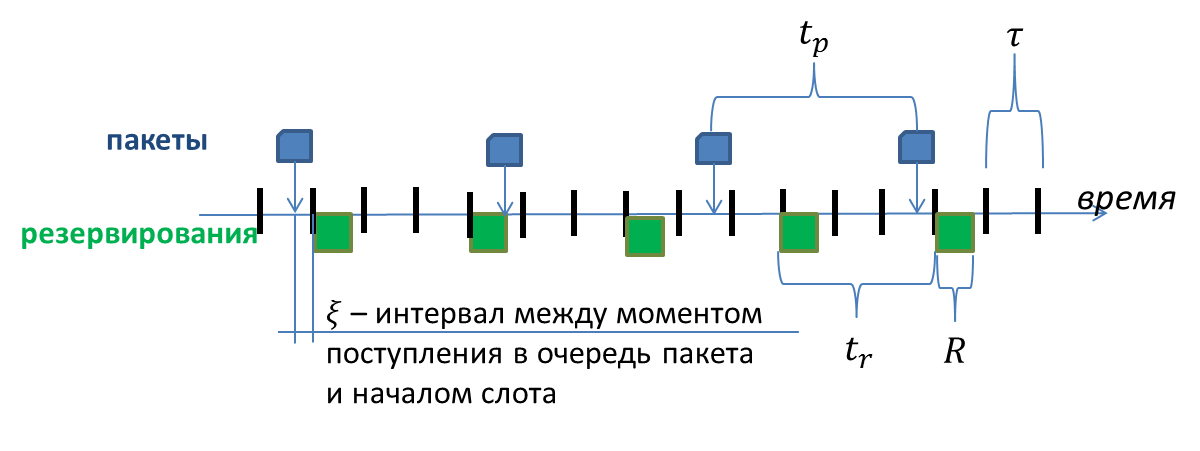
\includegraphics[width=0.8\textwidth]{pic/reserv.png} \\
    \caption{\label{fig:mcca:an:send} Передача пакетов с помощью периодических резервирований}
\end{figure}

Если очередь непуста, то возраст первого (самого старого) пакета обозначим как $h \tau+\xi$, где $h$ -- некоторое неотрицательное целое число. Так как пакеты поступают  в очередь строго периодически, число пакетов в очереди определяется величиной $\lfloor\frac{h}{t_p}\rfloor+1$, где $\lfloor x \rfloor$ равно целой части $x$, а возраст $i$-ого пакета равен $[h - (i-1)t_p ]\tau + \xi$ -- см. рис.~\ref{fig:mcca:an:queue}. Доопределим $h$ для тех случаев, когда пакета в очереди нет: $h<0$, $|h \tau+\xi|$ -- время до следующего поступления пакета в очередь.

\begin{figure}
 \centering
      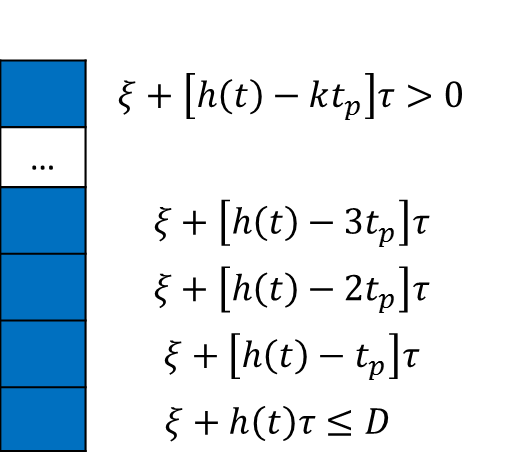
\includegraphics[width=0.32\textwidth]{pic/queue.png} \\
     \caption{\label{fig:mcca:an:queue}  Время ожидания пакетов в очереди}
 \end{figure}

Такое определение величины $h$ позволяет представить передачу пакетов с помощью периодических MCCA-резервирований одномерным марковским процессом $J(t)$ с состоянием системы $h(t)$ и дискретным временем, единица которого равна $t_r$ слотов, а моменты  $t$ и $t+1$  соответствуют началам двух последовательных зарезервированных интервалов -- см. рис.~\ref{fig:mcca:an:send}.

Опишем множество состояний процесса. Минимальное значение $h(t)$ равно $t_r - t_p$. Это значение достигается в момент $t+1$, когда пакет поступает в пустую очередь в слоте, предшествующем моменту $t$, и успешно передается в момент $t$. Очевидно, что максимальное значение $h(t)$ равно $d=\lfloor \frac{D-\xi}{\tau}\rfloor$.

Опишем возможные одношаговые переходы между состояниями процесса.

Пусть $0 \leq h(t), h(t)+t_r\leq d$. Тогда возможны 2 типа переходов.

 \begin{description}
   \item[Обслуживаемый пакет покидает очередь.] Так как возраст следующего пакета меньше на $t_p$ слотов, а единица модельного времени равна $t_r$ слотам, то с вероятностью $p$ успешной попытки передачи система переходит в состояние  $h(t+1) = h(t) - t_p + t_r$.
   \item[Обслуживаемый пакет остается в очереди.] С вероятностью $1-p$ попытка передачи оказалась неудачной, и к моменту $t+1$ возраст пакета увеличивается на $t_r$ слотов, т.е. система переходит в состояние $h(t+1)=h(t)+t_r$.
 \end{description}

Пусть $h(t) < 0$. Тогда пакета в очереди нет, и к моменту $t+1$ время до прихода пакета уменьшится на величину $t_r$, а если пакет придет, то его возраст будет равен $\xi + [t_r+h(t)]\tau$. В любом случае система переходит в состояние  $h(t+1)=h(t)+t_r$ с вероятностью 1.

Если $h(t)+t_r > d$, то вне зависимости от успеха попытки передачи пакета его обслуживание прекращается, так как в момент $t+1$ его возраст превысит допустимый. Система переходит в состояние $h(t+1) = h(t) - t_p + t_r$ с вероятностью 1.

Таким образом, из состояния $h-t_r$ система переходит в состояние $h$ с вероятностью $\alpha_h$, где
\[
\alpha_h = \left\{\begin{array}{ll}
    0,  &   h < -t_p+2t_r,  \\
    1-p,	&    t_r\leq h \leq d,      \\
    1,	&    -t_p+2t_r \leq h < t_r.
    \end{array} \right.
\]
Аналогично, из состояния $h+t_p-t_r$ система переходит в состояние $h$ с вероятностью $\beta_h$, где
\[
 \beta_h = \left\{ \begin{array}{ll}
    0,      &   h > d-t_p + t_r, \\
    p,    &	h \leq d-t_p,      \\
    1,      &	d-t_p < h \leq d - t_p + t_r.
    \end{array} \right.
\]

Пусть $\pi_{h}$, $h \in \{-t_p+t_r, \ldots, d\}$, -- стационарные вероятности состояний процесса $J(t)$. Тогда система уравнений для стационарных вероятностей записывается как

\begin{equation}\label{eq:mcca:system}
    \left\{
    \begin{array}{l}
    \pi_{h}= \alpha_h \cdot \pi_{h-t_r} + \beta_h \cdot \pi_{h+t_p-t_r}, h \in \{-t_p+t_r, \ldots, d\}, \\
    \sum \limits_{h=-t_p+t_r}^{d} \pi_{h} = 1.
    \end{array}
    \right.
\end{equation}

Решая систему линейных уравнений (\ref{eq:mcca:system}), получаем значения $\pi_{h}$ стационарных вероятностей состояний процесса.

Очевидно, что долю потеряных пакетов можно определить как отношение среднего числа  отброшенных за единицу времени пакетов к среднему числу поступивших пакетов. Пакет отбрасывается с вероятностью $1-p$ после передачи пакета из любого такого состояния  $h$, что $h+t_r> d$. Так как среднее число пакетов, поступивших за единицу времени, равно $t_r/t_p$, то доля потерянных пакетов определяется следующим выражением:
\begin{equation*}
   PLR=(1-p) t_p/t_r\sum_{i = d - t_r+1}^{d} p_{i}.
\end{equation*}

\subsection{Численные результаты}
Используя разработанную аналитическую модель, исследуем, как выбор периода резервирований влияет на долю потерянных пакетов. На рис.~\ref{fig:mcca:an:results:plr_vs_tc} приведены результаты, полученные для интервала $t_p^* = 20$~мс между пакетами, типичного для голосового трафика, сгенерированного кодеком G.729, вероятности успешной попытки передачи пакета $p = 0,7$ и смещения $\xi=0$, которое получается, если протокол резервирует первый интервал времени сразу после поступления пакета в очередь.

\begin{figure}[!htbp]
\centering
    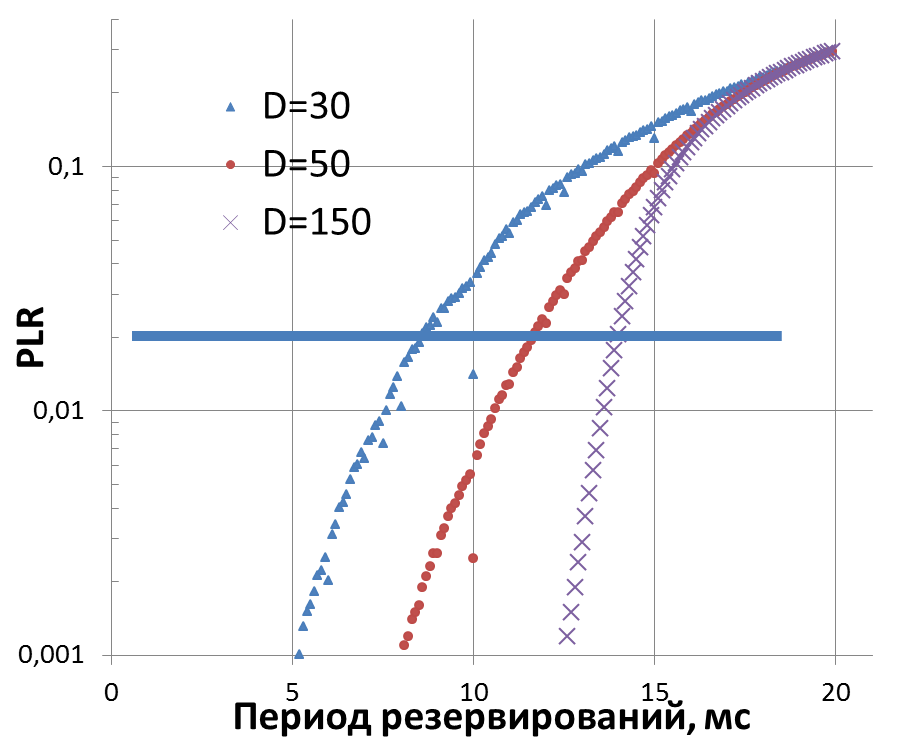
\includegraphics[width=0.7\textwidth]{pic/results.png} \\
    \caption{\label{fig:mcca:an:results:plr_vs_tc} $PLR(t_r^*)$ при $t_p^* = 20$~мс, $p = 0,7$.}
\end{figure}

При  $t_r^* = t_p^*$ период резервирований совпадает с интервалом поступления пакетов, т.е. на один пакет приходится ровно одно резервирование (одна попытка передачи), доля потерянных пакетов равна $1-p=0,7$ независимо от ограничения на максимально допустимое время доставки  $D_{QoS}$. Уменьшение $t_r^*$ и повышение допустимого времени доставки $D_{QoS}$  уменьшают долю потерянных пакетов, так как более частые резервирования предоставляют в среднем большее число попыток передачи для каждого пакета, а увеличение допустимого времени доставки позволяет воспользоваться этими попытками.

Из полученных результатов видна особенность функции $PLR(t_r^*)$: она не является монотонной ни в одной точке по следующим причинам.
Начнем с того, что построенная модель позволяет получить значения $PLR(t_r^*)$ только в таких точках, что $\frac{t_r^*}{t_p^*}$ является рациональным числом. Далее заметим, что средний интервал времени от момента поступления пакета в очередь до первого резервирования равен $\xi+\frac{t_r-1}{2}\tau=\xi+\frac{t_r^*-\tau}{2}$ и немонотонно зависит от $t_r^*$, так как $\tau(t_r^*)$ -- не монотонна. Чем этот интервал меньше, тем больше попыток приходится на пакет для его передачи. Очевидно, что при  $\xi=0$ и $t_r^*=\tau$ (т.е. $t_r^* = \frac{t_p^*}{k}, k \in N$)  интервал минимален, и  $PLR(t_r^* = \frac{t_p^*}{k})$ имеет локальный минимум. На графике это точки $t_r^*=10; 5$ мс.

<<Глубина>> этого минимума зависит от многих факторов.

Во-первых, она зависит от $\tau$. Если $\tau = t_r$ и  $\xi=0$, то первое резервирование всегда следует сразу за поступлением пакета в очередь. Это значит, что за время нахождения любого пакета в очереди совершается $1+d/t_r$ попыток передачи пакета. В то же время, если $\tau \ll t_r$, то только части пакетов соответствует $1+d/t_r$ попыток передачи, а остальным -- всего $d/t_r$ попыток.

Во-вторых, при увеличении допустимого времени доставки и, соответственно, числа попыток передач, совершаемых, пока пакет находится в очереди, вклад дополнительной попытки передачи уменьшается. Поэтому при больших $D$ функция ведет себя почти монотонно.

Используя предварительно вычисленную таблицу значений $PLR(t_r^*)$, станция может быстро подобрать необходимый период резервирований, обеспечивающий передачу пакетов с требуемым качеством обслуживания при минимальном потреблении канальных ресурсов.

